%% Does Your AI Coding Plan Still Buy What It Used To?
%% IEEE conference format (IEEEtran). Build: `just paper` or scripts/build.sh
\documentclass[conference]{IEEEtran}
\IEEEoverridecommandlockouts

\usepackage{cite}
\usepackage{amsmath,amssymb,amsfonts,amsthm}
\usepackage{algorithm}
\usepackage{algpseudocode}
\usepackage{graphicx}
\usepackage{booktabs}
\usepackage{siunitx}
\usepackage{listings}
\usepackage{xcolor}
\usepackage{tikz}
\usetikzlibrary{positioning,arrows.meta,fit,backgrounds}
\usepackage[hidelinks]{hyperref}
\usepackage{url}
\usepackage{balance}

% GENERATED by scripts/figures.py -- do not edit by hand.
\newcommand{\QstarDrop}{99}
\newcommand{\QstarRel}{0.014}
\newcommand{\alphaC}{3.5}
\newcommand{\alphaFat}{1.3}
\newcommand{\alphaThin}{2.5}
\newcommand{\canaryAlarms}{0}
\newcommand{\canaryArl}{200}
\newcommand{\canaryCycles}{10}
\newcommand{\canaryFirstDay}{2026-09-07}
\newcommand{\canaryLastDay}{2026-09-25}
\newcommand{\canaryPzero}{0.95}
\newcommand{\canarySolved}{10}
\newcommand{\codexCHatDeliveredK}{83.1}
\newcommand{\codexCHatFrozenK}{83.2}
\newcommand{\codexDiffHi}{+8}
\newcommand{\codexDiffLo}{-80}
\newcommand{\codexDiffPoint}{-36}
\newcommand{\codexMeterEnd}{4}
\newcommand{\codexMeterRes}{1}
\newcommand{\codexMeterStart}{1}
\newcommand{\codexMeterWindowDays}{7}
\newcommand{\codexModel}{gpt-6.1-sol}
\newcommand{\codexNRuns}{48}
\newcommand{\codexPostResetMeter}{0}
\newcommand{\codexProbeAtFull}{8}
\newcommand{\codexProbeCycles}{1678}
\newcommand{\codexProbeDutyDays}{8.4}
\newcommand{\codexProbeHours}{10}
\newcommand{\codexProbePerPoint}{17.5}
\newcommand{\codexProbeQ}{1748}
\newcommand{\codexProbeSessions}{6}
\newcommand{\codexProbeTokK}{79.1}
\newcommand{\codexReps}{3}
\newcommand{\codexSHatDelivered}{100}
\newcommand{\codexSHatFrozen}{100}
\newcommand{\codexTokMillions}{4.1}
\newcommand{\codexVerifyDate}{2026-10-02}
\newcommand{\codexVerifyPass}{4}
\newcommand{\codexVerifyRuns}{4}
\newcommand{\copilotVerifyCalls}{3}
\newcommand{\copilotVerifyDate}{2026-09-06}
\newcommand{\copilotVerifyOraclePass}{3}
\newcommand{\cpsRatio}{2.3}
\newcommand{\eGain}{40}
\newcommand{\epsChange}{+25}
\newcommand{\gammaHill}{1.6}
\newcommand{\jevonsSlack}{+0.22}
\newcommand{\kReps}{3}
\newcommand{\kappaMarg}{6}
\newcommand{\multdlnP}{1.00}
\newcommand{\multdlnQ}{0.70}
\newcommand{\multdlnc}{2.00}
\newcommand{\multdlne}{0.60}
\newcommand{\multdlns}{1.25}
\newcommand{\multdlntau}{2.60}
\newcommand{\nReqFifty}{23}
\newcommand{\nReqTen}{999}
\newcommand{\nReqThirty}{87}
\newcommand{\nReqTwenty}{223}
\newcommand{\pSolve}{0.45}
\newcommand{\pilotCHatDelivered}{0.242}
\newcommand{\pilotCHatFrozen}{0.231}
\newcommand{\pilotCostTotal}{11.29}
\newcommand{\pilotDate}{2026-09-05}
\newcommand{\pilotDiffHi}{+0.017}
\newcommand{\pilotDiffLo}{-0.004}
\newcommand{\pilotDiffP}{0.11}
\newcommand{\pilotDiffPoint}{+0.007}
\newcommand{\pilotNRuns}{48}
\newcommand{\pilotNTasks}{8}
\newcommand{\pilotProbeMinutes}{58}
\newcommand{\pilotProbeQSum}{6}
\newcommand{\pilotProbeSessions}{2}
\newcommand{\pilotReps}{3}
\newcommand{\pilotSHatDelivered}{100}
\newcommand{\pilotSHatFrozen}{100}
\newcommand{\priceRef}{20}
\newcommand{\rdlnP}{+0.00}
\newcommand{\rdlnQ}{-0.36}
\newcommand{\rdlnc}{+0.69}
\newcommand{\rdlne}{-0.51}
\newcommand{\rdlns}{+0.22}
\newcommand{\rdlntau}{+0.96}
\newcommand{\runsTen}{5992}
\newcommand{\scenDelta}{0.83}
\newcommand{\scenHalfLife}{10.1}
\newcommand{\scenLoss}{56}
\newcommand{\scenRatio}{44}
\newcommand{\scenTotal}{-0.83}
\newcommand{\scendlnP}{+0.0000}
\newcommand{\scendlnQ}{-0.3567}
\newcommand{\scendlnc}{+0.6931}
\newcommand{\scendlne}{-0.5108}
\newcommand{\scendlns}{+0.2231}
\newcommand{\scendlntau}{+0.9555}
\newcommand{\sigLog}{0.8}
\newcommand{\tauGrowth}{2.6}
\newcommand{\tauStar}{109}
\newcommand{\thetaRet}{2.5}
\newcommand{\varUnit}{2.12}


\theoremstyle{plain}
\newtheorem{proposition}{Proposition}
\newtheorem{corollary}{Corollary}
\theoremstyle{definition}
\newtheorem{definition}{Definition}

\definecolor{lstbg}{HTML}{F7F7F5}
\definecolor{lstkw}{HTML}{1F4E79}
\definecolor{lstcm}{HTML}{6B7280}
\lstset{
  basicstyle=\ttfamily\scriptsize,
  backgroundcolor=\color{lstbg},
  keywordstyle=\color{lstkw}\bfseries,
  commentstyle=\color{lstcm}\itshape,
  stringstyle=\color{lstkw},
  breaklines=true, showstringspaces=false,
  frame=leftline, framerule=0.8pt, rulecolor=\color{lstcm},
  xleftmargin=6pt, framexleftmargin=4pt, aboveskip=4pt, belowskip=2pt,
}

\newcommand{\NQU}{\ensuremath{\mathrm{NQU}}}
\newcommand{\RTP}{\ensuremath{\mathrm{RTP}}}
\newcommand{\CPS}{\ensuremath{\mathrm{CPS}}}
\newcommand{\EPS}{\ensuremath{\mathrm{EPS}}}
\newcommand{\CPPI}{\ensuremath{\mathrm{CPPI}}}
\newcommand{\eqdef}{\ensuremath{\triangleq}}

\begin{document}

\title{Does Your AI Coding Plan Still Buy What It Used~To? \\
A Purchasing-Power Index for Agentic Coding Subscriptions}

\author{\IEEEauthorblockN{Lucas Andrade Zanetti}
\IEEEauthorblockA{\textit{Faculdade de Ci\^{e}ncias e Tecnologias em Engenharia (FCTE)} \\
\textit{Universidade de Bras\'{i}lia} \\
Bras\'{i}lia, Brazil \\
landradezanetti@gmail.com}}

\maketitle

\begin{abstract}
Developers routinely report that their fixed-price AI coding subscription
``does less than it used to,'' while vendors report monotonically improving
benchmark scores. We show that both claims can be simultaneously true, and
that the disagreement is a measurement failure rather than a dispute about
facts: public benchmarks are \emph{capability-denominated} (they price a
model), whereas a subscription is \emph{quota-denominated} (it prices an
entitlement consumed by an agent harness whose appetite is itself drifting).
We define the Real Task Purchasing power of a plan, $\RTP = Qs/c$, and derive
an exact additive decomposition of its log change into four channels ---
entitlement, capability, consumption and price --- of which only price is
publicly observable. Three structural results follow. First, whenever the
elasticity of solve rate with respect to token budget falls below one ---
which concave test-time scaling guarantees --- the quota cost per solved task
must rise, so capability gains are bought at a worsening exchange rate.
Second, we give a falsifiable Jevons condition under which energy per solved
task increases despite falling energy per token. Third, a simple
retention--cost model shows that compressing quota is the profit-maximising
response to fat-tailed agentic usage, so devaluation is a rational vendor
behaviour rather than an accusation. We then specify a reproducible
measurement protocol --- a normalised quota unit, an empirical entitlement
probe, a frozen harness, a drift canary, and pre-registered hypotheses ---
and report a design analysis showing that resolving a $10\%$ change in plan
value needs a basket of roughly \nReqTen{} tasks. An individual developer's
lived experience is therefore underpowered by about two orders of magnitude,
which explains why the perception gap persists and why a shared index is
needed. The design-analysis numbers are outputs of a declared simulation, not
measurements of any plan; a small real pilot of a reference implementation,
run on the author's own accounts, shows that the instrument works end to end
and how underpowered a single developer's sample is, but it does not
measure plan value.
\end{abstract}

\begin{IEEEkeywords}
AI coding assistants, agentic software engineering, cost-aware evaluation,
benchmarking, index numbers, energy efficiency, LLM inference, software
economics.
\end{IEEEkeywords}

\section{Introduction}

A recurring complaint has followed every generation of commercial AI coding
tools: \emph{the plan I pay for feels worse than it did six months ago}.
The complaint is usually met with a rebuttal that is also true --- coding
benchmark scores have risen sharply and continue to
rise~\cite{jimenez2024swebench,jain2025livecodebench}. Both sides argue past
each other because they are quoting prices in different currencies.

A published benchmark score answers a \emph{capability-denominated} question:
given an unbounded or unstated budget, what fraction of tasks does this model
solve? A subscriber asks a \emph{quota-denominated} question: given the
entitlement my \$$X$/month buys, how much shipped engineering work can I get
before I am throttled? These two quantities are connected by three factors
that all drift, mostly silently:

\begin{enumerate}
\item the \textbf{entitlement} $Q$ the plan grants, expressed in units the
      vendor defines and may redefine (messages, tokens, credits, weekly
      caps, per-model multipliers);
\item the \textbf{capability} $s$ of whichever model the plan routes to on
      the day you use it --- which is not contractually fixed, and which
      measurably moves over time~\cite{chen2024drift};
\item the \textbf{consumption} $c$ that a modern agent harness burns to
      attempt one task, which has grown by orders of magnitude as
      chain-of-thought, tool loops, repository search and test-repair cycles
      became standard practice~\cite{wei2022cot,snell2024scaling,yang2024sweagent}.
\end{enumerate}

Only the price $P$ is contractual and public. The other three are private to
the vendor, and the product of the four is what the user actually buys. A
plan can therefore be devalued to half its former usefulness without a single
line of the pricing page changing --- the same way a currency can be debased
without altering the number printed on the note.

This paper takes the folk question in its title seriously enough to make it
measurable. We treat a coding subscription as a good whose real price should
be tracked with the machinery economists use for consumer
prices~\cite{fisher1922index,ilo2004cpi}: a fixed basket of tasks, an index
over time, an explicit substitution-bias analysis, and a hedonic adjustment
for quality. The novel object is the denominator: instead of pricing the
basket in dollars, we price it in the plan's own entitlement.

\subsection{Contributions}

\begin{itemize}
\item \textbf{A value model} for coding subscriptions
      (Section~\ref{sec:model}) built on a \emph{Normalised Quota Unit}
      that makes heterogeneous, undisclosed meters comparable across vendors
      and across time, together with an exact additive four-channel
      decomposition of the change in value (Proposition~\ref{prop:decomp}).
\item \textbf{Three structural results} (Section~\ref{sec:why}) explaining
      why value can fall while capability rises: a concavity result forcing
      quota cost per solved task upward
      (Proposition~\ref{prop:elasticity}); a falsifiable Jevons condition
      for energy per solved task (Proposition~\ref{prop:jevons}); and a
      vendor-side result showing that quota compression maximises profit
      under fat-tailed agentic usage (Proposition~\ref{prop:vendor}).
\item \textbf{A measurement protocol}, \textsc{Planmeter}
      (Section~\ref{sec:protocol}): basket construction with contamination
      control, harness freezing, an entitlement saturation probe, a
      capability-drift canary, an instrumented run record, and five
      pre-registered hypotheses.
\item \textbf{A design analysis} (Section~\ref{sec:sim}) giving closed-form
      sample sizes for the index and showing that a solo developer's
      experience cannot statistically resolve the devaluation they perceive.
\item \textbf{A reference implementation and a small real pilot}
      (Section~\ref{sec:harness}): an open harness with adapters for three
      coding-assistant clients, run end to end on the author's own accounts,
      whose main finding is how differently each client exposes consumption.
\item \textbf{A disclosure artifact}, the \emph{Plan Value Card}
      (Section~\ref{sec:card}), in the spirit of model
      cards~\cite{mitchell2019modelcards} and
      datasheets~\cite{gebru2021datasheets}.
\end{itemize}

\subsection{What this paper does and does not claim}
\label{sec:scope}

This is an instrument paper. Its contribution is a theory of the quantity to
be measured and a protocol for measuring it. Every numeric value reported in
Section~\ref{sec:sim} is the output of a simulation whose parameters are
declared in Table~\ref{tab:scenario}; none of them is a measurement of any
commercial plan, and none should be cited as one. Section~\ref{sec:harness}
separately reports a small \emph{measured} pilot of the reference
implementation, run on the author's own accounts and labelled as such; it is
far too underpowered to estimate plan value (Appendix~\ref{app:power}) and
reproduces no vendor price or quota. We do not reproduce pricing tables that
would be stale before publication, and do not assert that any observed
devaluation has occurred.
Section~\ref{sec:ethics} states the terms-of-service boundary that a
deployment of this protocol must respect.

\section{Background and Related Work}

\subsection{Capability-denominated benchmarks}
Code benchmarks evolved from function-level synthesis
(HumanEval~\cite{chen2021humaneval}, MBPP~\cite{austin2021mbpp}) to
repository-level issue resolution
(SWE-bench~\cite{jimenez2024swebench} and its human-validated
subset~\cite{openai2024swebenchverified}), to contamination-resistant rolling
sets~\cite{jain2025livecodebench} and terminal-native agent
tasks~\cite{terminalbench2025,aider2024polyglot}. Scores are reported per
\emph{model}, but they are produced by a \emph{scaffold} ---
SWE-agent~\cite{yang2024sweagent}, OpenHands~\cite{wang2025openhands} --- and
scaffold changes move scores as much as model changes do. Budgets are usually
unreported, so the same headline number can correspond to wildly different
resource consumption.

\subsection{Cost-aware evaluation}
Kapoor et al.~\cite{kapoor2024agents} make the case directly: agent
evaluations that ignore cost reward wasteful scaffolds, and accuracy should
be read on a cost--accuracy Pareto frontier. FrugalGPT~\cite{chen2023frugalgpt}
optimises cascades against dollar cost, and HELM~\cite{liang2023helm} reports
efficiency alongside accuracy. All of these denominate cost in
\emph{API dollars}. That is the right unit for someone paying per token and
the wrong unit for the tens of millions of developers on flat-rate plans,
whose binding constraint is an entitlement they cannot observe. To our
knowledge no prior work measures the subscription rather than the model.

\subsection{Capability drift and deprecation}
Chen et al.~\cite{chen2024drift} document measurable behavioural change in a
fixed commercial endpoint over months. Contemporary practice adds two further
sources of drift invisible to the user: server-side routing among models of
different cost, and deprecation of the endpoint a longitudinal study was
anchored to. Section~\ref{sec:infeasible} shows that the latter is not merely
inconvenient --- it makes an entire family of index numbers uncomputable.

\subsection{Energy of inference}
Per-token inference energy has fallen substantially through batching, paged
attention~\cite{kwon2023vllm}, speculative decoding~\cite{leviathan2023speculative}
and hardware turnover, and careful measurement methodology exists at the
request level~\cite{samsi2023watts,luccioni2024powerhungry} and the
lifecycle level~\cite{strubell2019energy,patterson2021carbon,luccioni2023bloom,henderson2020systematic}.
Aggregate data-centre projections~\cite{masanet2020recalibrating,iea2025energyai}
nevertheless keep rising. This is the classic Jevons
structure~\cite{jevons1865coal}: efficiency per unit of consumption
increases, consumption increases faster. Section~\ref{sec:jevons} states the
condition in the units a developer cares about --- joules per solved task,
not joules per token.

\subsection{Productivity evidence}
Field studies of AI assistance report large task-level speedups in controlled
settings~\cite{peng2023copilot,brynjolfsson2025genai}, while a randomised
study of experienced maintainers on their own repositories found a
\emph{slowdown} despite participants believing they had been sped
up~\cite{metr2025slowdown}. That gap between perceived and measured value is
precisely the gap this paper instruments, and it motivates the hedonic
correction of Section~\ref{sec:hedonic}: a passing test is not the same as
accepted work.

\subsection{Index numbers, quality and information asymmetry}
We borrow directly from price-index practice: Laspeyres and Paasche forms and
the Fisher ideal index~\cite{fisher1922index,ilo2004cpi}, substitution
bias~\cite{boskin1996toward}, hedonic quality
adjustment~\cite{triplett2006hedonic}, and Nordhaus's long-run real price of
computation~\cite{nordhaus2007computing}. The market-design reading is
Akerlof's~\cite{akerlof1970lemons}: when only the seller can observe the
quality of the delivered good, buyers discount all sellers, and the honest
seller has no way to signal. A published index is exactly such a signalling
device. Versioning a bundled information good under heterogeneous
willingness-to-pay is the classic
treatment~\cite{shapiro1999information}; our Proposition~\ref{prop:vendor}
adds what happens when the usage distribution's tail is fattened by
autonomous agents.

\begin{figure}[t]
\centering
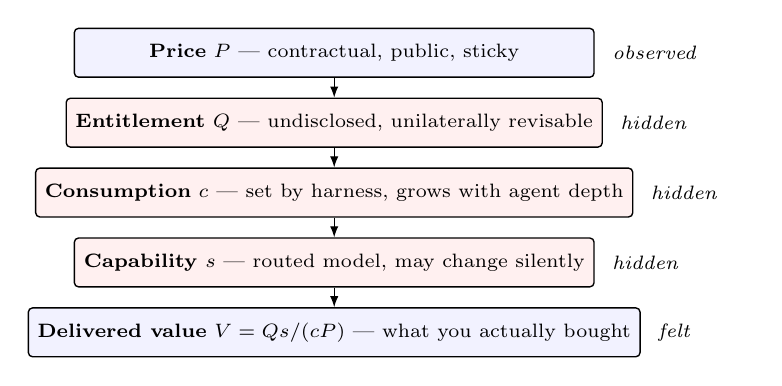
\begin{tikzpicture}[
  font=\scriptsize,
  layer/.style={draw, rounded corners=1.5pt, minimum width=6.6cm,
                minimum height=0.62cm, align=center, line width=0.5pt},
  obs/.style={layer, fill=blue!5},
  hid/.style={layer, fill=red!6},
  lbl/.style={font=\scriptsize\itshape, anchor=west}
]
\node[obs] (p) {\textbf{Price} $P$ --- contractual, public, sticky};
\node[hid, below=2.5mm of p] (q) {\textbf{Entitlement} $Q$ --- undisclosed, unilaterally revisable};
\node[hid, below=2.5mm of q] (c) {\textbf{Consumption} $c$ --- set by harness, grows with agent depth};
\node[hid, below=2.5mm of c] (s) {\textbf{Capability} $s$ --- routed model, may change silently};
\node[obs, below=2.5mm of s] (v) {\textbf{Delivered value} $V=Qs/(cP)$ --- what you actually bought};
\draw[-{Latex[length=1.4mm]}] (p) -- (q);
\draw[-{Latex[length=1.4mm]}] (q) -- (c);
\draw[-{Latex[length=1.4mm]}] (c) -- (s);
\draw[-{Latex[length=1.4mm]}] (s) -- (v);
\node[lbl, right=1mm of p.east, text width=1.1cm] {observed};
\node[lbl, right=1mm of q.east, text width=1.1cm] {hidden};
\node[lbl, right=1mm of c.east, text width=1.1cm] {hidden};
\node[lbl, right=1mm of s.east, text width=1.1cm] {hidden};
\node[lbl, right=1mm of v.east, text width=1.1cm] {felt};
\end{tikzpicture}
\caption{The value stack of a coding subscription. The user contracts on the
only layer that does not move, experiences the bottom layer, and cannot
observe the three layers in between. Every published benchmark measures a
projection of the fourth layer alone.}
\label{fig:stack}
\end{figure}

\section{A Value Model for Coding Subscriptions}
\label{sec:model}

\subsection{Objects}

\begin{definition}[Task basket]
A basket $\mathcal{B}=\{(b_1,w_1),\dots,(b_n,w_n)\}$, $\sum_i w_i = 1$, where
each $b_i$ is a software-engineering task pinned to a repository commit and
equipped with a machine-checkable oracle (a test suite, a differential
oracle, or a build-and-lint gate). Weights encode the mix of work a given
population of developers actually does.
\end{definition}

\begin{definition}[Epoch, plan, harness]
An epoch $t$ is a measurement window (we use a calendar month). A plan
$p$ has public price $P(p,t)$ per epoch. A harness $h$ is the complete
client-side configuration: agent loop, tool set, context policy, retry
policy, step limit, temperature, and the model selector the plan exposes.
\end{definition}

A single \emph{run} of $b_i$ under $(p,h,t)$ yields four observables:
$x_i\in\{0,1\}$ oracle success; $u_i>0$ quota consumed;
$\tau_i>0$ tokens consumed, split into prefill, decode, cached-read and
cached-write classes; and $\kappa_i\in[0,1]$ a review-quality score.

\subsection{The Normalised Quota Unit}

Vendors meter in incomparable units, redefine them, and apply per-model
multipliers. We therefore define the unit endogenously.

\begin{definition}[\NQU]
Fix a calibration task $b_0$ and a reference harness $h_0$, both frozen for
the life of the study. One \NQU{} is the quota consumed by one execution of
$(b_0,h_0)$. The entitlement $Q(p,t)$ is the number of such executions
completable within one billing epoch before the plan throttles.
\end{definition}

This makes $Q$ an \emph{observable} even when the vendor discloses nothing:
it is measured, not read off a pricing page (Algorithm~\ref{alg:probe}).
It also makes meter redefinition detectable, because \NQU{} is anchored to
$b_0$'s token counts, which the API still reports.

\subsection{Purchasing power}

Write $\bar{x}_i,\bar{u}_i$ for means over $k$ repetitions. Define basket
solve rate and basket consumption per attempt:
\begin{equation}
s(t) \eqdef \sum_i w_i \bar{x}_i(t), \qquad
c(t) \eqdef \sum_i w_i \bar{u}_i(t) .
\end{equation}
The quota cost of one unit of delivered work and the amount of work a plan
buys per epoch are then
\begin{equation}
\CPS(t) \eqdef \frac{c(t)}{s(t)}, \qquad
\RTP(p,t) \eqdef \frac{Q(p,t)\, s(t)}{c(t)} ,
\label{eq:rtp}
\end{equation}
in $\NQU$ per solve and in solves per epoch respectively.
$\RTP$ is the honest answer to
``what does this plan do for me this month.'' Normalising by price gives
value per dollar,
\begin{equation}
V(p,t) \eqdef \frac{\RTP(p,t)}{P(p,t)} = \frac{Q(p,t)\,s(t)}{c(t)\,P(p,t)} .
\label{eq:value}
\end{equation}

\begin{definition}[Coding-Plan Purchasing-power Index]
$\CPPI(p,t;t_0) \eqdef V(p,t)/V(p,t_0)$, with continuously compounded
\emph{debasement rate}
$\delta \eqdef -\ln \CPPI(p,t;t_0)/(t-t_0)$.
\end{definition}

A plan with $\delta = 0.30\,\text{yr}^{-1}$ loses a quarter of its real value
per year at an unchanged sticker price. Reporting $\delta$ alongside $P$ is
the central practical proposal of this paper.

\subsection{The four channels}

\begin{proposition}[Exact additive decomposition]
\label{prop:decomp}
For any two epochs,
\begin{equation}
\underbrace{\Delta \ln V}_{\text{value}} =
\underbrace{\Delta \ln Q}_{\text{entitlement}} +
\underbrace{\Delta \ln s}_{\text{capability}} -
\underbrace{\Delta \ln c}_{\text{consumption}} -
\underbrace{\Delta \ln P}_{\text{price}} .
\label{eq:decomp}
\end{equation}
\end{proposition}
\begin{IEEEproof}
Immediate from~\eqref{eq:value} and the additivity of $\ln$ over products
and quotients. The decomposition is exact, not a first-order approximation,
which is why we work in logs throughout.
\end{IEEEproof}

Equation~\eqref{eq:decomp} is the analytical core of the paper. It says the
four causes of felt devaluation are separable and individually estimable, and
it immediately explains the public argument: vendors quote the second term,
users feel the sum, and the first and third terms --- the ones with the
largest recent movement --- are unobservable to everyone outside the vendor.

\subsection{Quality adjustment}
\label{sec:hedonic}

A green test suite is a lower bound on value, not value. Following hedonic
practice~\cite{triplett2006hedonic} we replace $s$ with a quality-weighted
solve rate
\begin{equation}
\tilde{s}(t) \eqdef \sum_i w_i \, \overline{x_i \kappa_i}(t),
\end{equation}
where $\kappa_i$ scores the accepted patch on diff minimality, absence of
dead or duplicated code, test quality, and adherence to repository
convention. $\kappa$ may be produced by a rubric-driven LLM
judge~\cite{zheng2023judge} provided the judge model and prompt are frozen
for the life of the study and calibrated against human review on a held-out
sample; a drifting judge silently contaminates the capability channel.
Reporting both $s$ and $\tilde{s}$ separates ``it passes'' from ``I would
merge it,'' the distinction that~\cite{metr2025slowdown} suggests dominates
real developer time.

\subsection{Substitution bias and index infeasibility}
\label{sec:infeasible}

Users re-optimise when quota binds: they switch to a cheaper model tier,
shorten context, disable extended reasoning, or batch work differently. A
fixed-harness index therefore overstates the loss, exactly as a fixed-basket
consumer index overstates inflation~\cite{boskin1996toward}. We report both
bounds. With $h_{t_0}$ the base-epoch harness and $h_t$ the epoch-$t$
re-optimised harness,
\begin{equation}
L(t) = \frac{V(h_{t_0},t)}{V(h_{t_0},t_0)}, \quad
Pa(t) = \frac{V(h_{t},t)}{V(h_{t},t_0)},
\end{equation}
with the Fisher ideal index $F(t)=\sqrt{L(t)\,Pa(t)}$
\cite{fisher1922index} as the headline figure.

\begin{proposition}[Infeasibility under deprecation]
\label{prop:deprecation}
If the model or endpoint available at $t_0$ is withdrawn before $t$, the
denominator $V(h_t,t_0)$ is unmeasurable and $Pa(t)$, hence $F(t)$, does not
exist. Only the Laspeyres bound survives, and only for as long as the
base-epoch harness remains runnable.
\end{proposition}

This is not a technicality. It means a vendor that retires old endpoints on
a cadence shorter than the study window destroys the comparability of its own
product over time --- the good whose price we are trying to track ceases to
exist. Long-run measurement of AI subscriptions requires archived reference
endpoints in the way metrology requires reference artefacts. We return to
this in Section~\ref{sec:discussion}.

\section{Why Value Can Fall While Capability Rises}
\label{sec:why}

\subsection{Concavity forces the unit cost of work upward}

Let $s(\tau)$ be the solve rate as a function of per-attempt token budget
$\tau$, and $\eta_{s,\tau} \eqdef (\mathrm{d}s/\mathrm{d}\tau)(\tau/s)$ its
elasticity.

\begin{proposition}[Rising cost per solved task]
\label{prop:elasticity}
$\dfrac{\mathrm{d}}{\mathrm{d}\tau}\left(\dfrac{\tau}{s(\tau)}\right) > 0
\iff \eta_{s,\tau} < 1$.
\end{proposition}
\begin{IEEEproof}
$\frac{\mathrm{d}}{\mathrm{d}\tau}\frac{\tau}{s}
= \frac{s - \tau s'}{s^2}
= \frac{1}{s}\left(1 - \eta_{s,\tau}\right)$, and $s>0$.
\end{IEEEproof}

\begin{corollary}
\label{cor:logscaling}
Under the log-linear test-time scaling regime reported for reasoning
models~\cite{snell2024scaling,deepseek2025r1}, $s \approx a + b\ln\tau$ gives
$\eta_{s,\tau} = b/s \to 0$ as $s$ saturates. Cost per solved task then grows
asymptotically linearly in the budget: every additional point of accuracy is
purchased at a strictly worse exchange rate than the last.
\end{corollary}

Fig.~\ref{fig:elasticity} makes the geometry concrete on a saturating curve
with shape parameter $\gamma=\gammaHill$. Unit cost is minimised at
$\tau^\star \approx \tauStar \times 10^3$ tokens per attempt and rises
monotonically thereafter; at a budget of $600\times10^3$ tokens --- ordinary
for a present-day repository-level agent run --- the cost per solved task is
already $\cpsRatio\times$ its minimum. The vendor's benchmark score and the
user's throughput are both moving, in opposite directions, for the same
reason.

\begin{figure*}[t]
\centering
\includegraphics[width=\textwidth]{figures/fig_elasticity.pdf}
\caption{Concave test-time scaling makes delivered work more expensive even
as accuracy improves. (a) A saturating solve-rate curve; the dashed line
marks unit elasticity. (b) The corresponding quota cost per solved task,
$\tau/s(\tau)$, which is minimised at $\tau^\star$ and increases without
bound. Agent harnesses operate far to the right of $\tau^\star$. Curve shape
is declared, not fitted to any vendor.}
\label{fig:elasticity}
\end{figure*}

\subsection{The iso-value map}

Holding price fixed, Proposition~\ref{prop:decomp} makes the trade-off
two-dimensional. Fig.~\ref{fig:isovalue} plots $\Delta\ln V$ over the
$(\Delta\ln s, \Delta\ln c)$ plane at an entitlement change of
$\Delta\ln Q = \scendlnQ$. The black contour is the break-even locus
$\Delta\ln s = \Delta\ln c - \Delta\ln Q$. Everything below and to the right
of it is the region a marketing page describes as progress and a user
experiences as loss. We call it the \emph{progress trap}: capability strictly
improves, delivered value strictly falls, and no party is lying.

\begin{figure}[t]
\centering
\includegraphics[width=\columnwidth]{figures/fig_isovalue.pdf}
\caption{Iso-value map. Blue is value gain, red is value loss, the black
contour is break-even. The marked point is the declared scenario of
Table~\ref{tab:scenario}: capability up $25\%$, consumption up $2\times$,
entitlement down $30\%$.}
\label{fig:isovalue}
\end{figure}

\subsection{Energy: a Jevons condition at the task level}
\label{sec:jevons}

Let $e(t)$ be the marginal energy per token of the serving stack and
$\bar\tau(t)$ the basket-mean tokens per attempt. Energy per solved task is
\begin{equation}
\EPS(t) = \frac{\bar\tau(t)\, e(t)}{s(t)} \quad [\si{\joule}/\text{solve}].
\end{equation}

\begin{proposition}[Task-level rebound]
\label{prop:jevons}
$\EPS$ increases between two epochs if and only if
\begin{equation}
\Delta \ln \bar\tau \;-\; \Delta \ln s \;>\; -\,\Delta \ln e .
\label{eq:jevons}
\end{equation}
That is: the environmental gain from serving efficiency is realised at the
task level only when per-token efficiency improves faster than agent
verbosity net of capability.
\end{proposition}

Condition~\eqref{eq:jevons} is falsifiable with the instrumentation of
Section~\ref{sec:protocol}: $\bar\tau$ and $s$ are measured directly, and
$e$ is bounded rather than asserted. We estimate $e$ bottom-up as
\begin{equation}
e \;=\; \mathrm{PUE}\cdot \overline{\mathrm{P}}_{\text{node}}
\left(\frac{\phi}{\Lambda_{\text{prefill}}}
    + \frac{1-\phi}{\Lambda_{\text{decode}}}\right) ,
\label{eq:energy}
\end{equation}
a token-mix average of the per-phase energies, with
$\overline{\mathrm{P}}_{\text{node}}$ the average node power, $\Lambda$ the
measured token throughput in each phase, and $\phi$ the prefill share --- reporting an interval over a declared range of batch sizes and
utilisations rather than a point estimate, following the methodology of
\cite{samsi2023watts,luccioni2024powerhungry,henderson2020systematic}.
Any study using~\eqref{eq:energy} must state that it is an external bound and
not a vendor disclosure. Fig.~\ref{fig:jevons} shows the rebound for the
declared scenario: a $\eGain\%$ reduction in energy per token is more than
cancelled by a $\tauGrowth\times$ growth in tokens per attempt, leaving
energy per solved task $\epsChange\%$ higher after twelve months. The slack
in~\eqref{eq:jevons} is $\jevonsSlack$; per-token efficiency would have had
to improve by that much again merely to hold the line.

\begin{figure*}[t]
\centering
\includegraphics[width=\textwidth]{figures/fig_jevons.pdf}
\caption{The Jevons structure at the task level under the declared scenario
of Table~\ref{tab:scenario}. (a) Per-token energy falls while tokens per
attempt rise faster; capability improves only modestly. (b) The product,
energy per \emph{solved task}, rises. Illustrative parameters, not
measurements.}
\label{fig:jevons}
\end{figure*}

\subsection{The vendor's side: compression is rational}

It is tempting to read devaluation as bad faith. A minimal model says
otherwise. Let per-subscriber usage $U$ follow a Pareto law with tail index
$\alpha$ and scale $u_m=1$ --- the standard shape once a minority of users
run autonomous agents overnight. The vendor sets a quota $Q$; marginal
serving cost is $\kappa$ per \NQU; retention is increasing and saturating in
generosity, $R(Q)=Q^\theta/(Q^\theta+Q_c^\theta)$. Expected profit per
subscriber is
\begin{equation}
\pi(Q) = R(Q)\,\bigl[P - \kappa\, m(Q)\bigr], \quad
m(Q) \eqdef \mathbb{E}\!\left[\min(U,Q)\right],
\end{equation}
with $m(Q) = 1 + \frac{1 - Q^{1-\alpha}}{\alpha-1}$ and
$m'(Q) = \Pr[U>Q] = Q^{-\alpha}$.

\begin{proposition}[Rational quota compression]
\label{prop:vendor}
Any interior optimum satisfies
\begin{equation}
\frac{R'(Q)}{R(Q)} \;=\; \frac{\kappa\, Q^{-\alpha}}{P - \kappa\, m(Q)} ,
\label{eq:foc}
\end{equation}
and an interior optimum exists precisely when $\alpha < 1+\theta$. Fattening
the usage tail (decreasing $\alpha$) raises the right-hand side pointwise
while leaving the left-hand side unchanged, so $Q^\star$ falls.
\end{proposition}
\begin{IEEEproof}
Differentiate $\ln \pi$ and set to zero to obtain~\eqref{eq:foc}. As
$Q\to\infty$, $R'/R \sim \theta Q_c^\theta Q^{-(1+\theta)}$ while the
right-hand side decays as $Q^{-\alpha}$; profit is eventually increasing in
$Q$ iff $1+\theta < \alpha$, which gives the existence condition. For the
comparative static, $\partial/\partial\alpha$ of the right-hand side is
negative for $Q>1$, so decreasing $\alpha$ shifts the crossing point left.
\end{IEEEproof}

Fig.~\ref{fig:vendor} solves~\eqref{eq:foc} numerically at
$P=\priceRef$, $\kappa=\kappaMarg$, $\theta=\thetaRet$. Moving the tail index
from $\alphaThin$ to $\alphaFat$ --- the qualitative effect of agentic use
arriving on a plan priced for chat use --- drives the optimal entitlement to
$\times\QstarRel$ of its former level. Two consequences follow. First,
subscribers are right that plans tighten and vendors are right that they must;
the conflict is structural. Second, because the tail is what makes flat-rate
unstable, flat-rate pricing for agentic workloads is a transitional regime,
not an equilibrium (Section~\ref{sec:discussion}).

\begin{figure}[t]
\centering
\includegraphics[width=\columnwidth]{figures/fig_vendor.pdf}
\caption{Profit-maximising entitlement as the usage distribution's tail
fattens, normalised to $Q^\star(\alpha=\alphaThin)$. Declared model
parameters; the qualitative direction, not the magnitude, is the result.}
\label{fig:vendor}
\end{figure}

\section{\textsc{Planmeter}: A Measurement Protocol}
\label{sec:protocol}

The model of Section~\ref{sec:model} is only useful if each of its four
channels can be estimated by an outside party with one ordinary account.
This section specifies how.

\subsection{Basket construction}

We stratify by the shape of work, not by language, because consumption scales
with agent depth rather than syntax:

\begin{itemize}
\item \textbf{S1 --- local repair} (weight $0.30$): single-file bug fix with a
      failing regression test; $\le 2$ tool calls expected.
\item \textbf{S2 --- feature} (weight $0.35$): multi-file change behind an
      existing interface, tests to be written by the agent.
\item \textbf{S3 --- migration} (weight $0.20$): mechanical but repository-wide
      change (API rename, dependency major bump) with a build-and-test gate.
\item \textbf{S4 --- long-horizon} (weight $0.15$): open-ended issue requiring
      reproduction, localisation, fix and test, capped at a declared step
      limit.
\end{itemize}

Three contamination controls are mandatory, following the reasoning
of~\cite{jain2025livecodebench}. (i) Tasks are drawn from commits dated after
the announced training cutoff of every model under test, and the basket rolls
forward each epoch with a frozen legacy arm retained for comparability.
(ii) A private hold-out third of the basket is never published; only aggregate
statistics from it are. (iii) Task statements are paraphrased and identifiers
in the prose (not the code) are perturbed, so verbatim-recall shortcuts fail.

\subsection{Freezing the harness}
\label{sec:harnessfix}

The most common way to ruin this measurement is to let the client improve
during the study. We pin the agent loop by commit hash, the tool schemas, the
system prompt, the context-compaction policy, the retry policy, the step
limit, and the decoding parameters. Two arms are then run every epoch:

\begin{itemize}
\item \textbf{frozen arm} ($h_{t_0}$) --- isolates vendor-side change; this is
      the arm that estimates $\Delta\ln s$ and $\Delta\ln c$ cleanly.
\item \textbf{as-delivered arm} ($h_t$) --- the vendor's current default
      client at its current defaults; this is what a user actually
      experiences, and its difference from the frozen arm is the value the
      \emph{tooling} added or destroyed independently of the model.
\end{itemize}

Reporting only the frozen arm attributes harness progress to the vendor's
model; reporting only the as-delivered arm hides model regressions behind
scaffold improvements. Both are required.

\subsection{Instrumentation}

Every run emits one JSON record. Token classes must be separated: cached
reads are typically an order of magnitude cheaper than fresh prefill, so a
harness change that improves cache hit rate looks like a capability gain if
they are pooled.

\begin{lstlisting}[language=,caption={Run record schema (one JSONL line per
run). Fields marked \texttt{null} when the vendor does not expose them.},
label={lst:record}]
{"run_id":"...","epoch":"2026-09","plan":"vendor-x/t2",
 "task":{"id":"S2-0417","stratum":"S2","repo":"org/repo",
   "commit":"9f1c...","rev":3},
 "harness":{"arm":"frozen","commit":"a17b...",
   "step_limit":40,"temp":0.0,"ctx":"summarize@0.7"},
 "model":{"advertised":"...","fingerprint":"...",
   "routed":null},
 "outcome":{"oracle_pass":true,"steps":17,
   "wall_s":412.6,"kappa":0.82,"judge":"judge-v1"},
 "tokens":{"prefill":184320,"decode":39114,
   "reasoning":22870,"cache_read":911002},
 "quota":{"meter_before":0.7314,"meter_after":0.7089,
   "consumed_nqu":1.83,"unit":"vendor-native"},
 "energy":{"model":"bottom-up-v2","j_lo":4.1e4,
   "j_hi":1.9e5}}
\end{lstlisting}

\subsection{Measuring an undisclosed entitlement}

$Q(p,t)$ is the quantity the vendor does not publish, and it is the one with
the largest recent movement. It can nevertheless be estimated by saturation
search on a single owned account.

\begin{algorithm}[t]
\caption{Entitlement saturation probe}
\label{alg:probe}
\begin{algorithmic}[1]
\Require calibration task $b_0$, reference harness $h_0$, plan $p$,
         epoch budget, duty-cycle limit $\rho$
\State $j \gets 0$; $\hat{Q} \gets 0$
\While{not throttled \textbf{and} epoch not exhausted}
  \State run $(b_0,h_0)$; record meter reading and latency
  \State $j \gets j+1$
  \If{response indicates rate limit or tier downgrade}
     \State record throttle type, reset horizon, and residual capability
     \State \textbf{break}
  \EndIf
  \State sleep to respect $\rho$ \Comment{never exceed documented limits}
\EndWhile
\State $\hat{Q} \gets j$ \Comment{in \NQU{} by construction}
\State \Return $\hat{Q}$, throttle class $\in$ \{hard stop, queue,
       silent model downgrade\}
\end{algorithmic}
\end{algorithm}

Three refinements matter. First, the throttle \emph{class} is itself a
finding: a plan that silently routes to a smaller model on exhaustion has not
reduced $Q$, it has reduced $s$ --- a different channel of
Equation~\eqref{eq:decomp} with different consequences for the user. Second,
many plans use rolling multi-scale windows (per-hour, per-day, per-week);
$\hat{Q}$ must therefore be reported per window, with the binding window
identified. Third, the probe is run at a low duty cycle at randomised times
of day, because entitlement in practice interacts with server load; see
Section~\ref{sec:ethics}.

\subsection{Capability-drift canary}

A small canary set of tasks with historically stable difficulty is run at
higher frequency than the full basket. Because we are watching a stream for
a step change rather than testing a fixed hypothesis, we use a one-sided
CUSUM~\cite{page1954cusum} on the canary solve rate with an alarm threshold
calibrated to a declared in-control false-alarm rate. Latency distributions
and response-format fingerprints are recorded as covariates. We stress that
these are \emph{signals}, not identification: a change in latency is
consistent with routing, load, or a serving-stack upgrade, and the protocol
reports the alarm and the covariates, never a claim about which model served
the request.

\subsection{Index computation}

\begin{algorithm}[t]
\caption{Epoch index computation}
\label{alg:index}
\begin{algorithmic}[1]
\Require basket $\mathcal{B}$, arms $\{h_{t_0},h_t\}$, repetitions $k$,
         base epoch $t_0$
\For{each arm $h$, task $b_i$, repetition $1..k$}
  \State execute; append run record (Listing~\ref{lst:record})
\EndFor
\State $\hat{s} \gets \sum_i w_i \bar{x}_i$;
       $\hat{\tilde{s}} \gets \sum_i w_i \overline{x_i\kappa_i}$;
       $\hat{c} \gets \sum_i w_i \bar{u}_i$
\State $\hat{Q} \gets$ Algorithm~\ref{alg:probe};
       $P \gets$ archived public price for epoch $t$
\State $\hat{V} \gets \hat{Q}\hat{s} / (\hat{c}P)$
\State bootstrap $B{=}10^4$ resamples \emph{over tasks} (not runs) for
       CI on $\ln\hat{V}$ \Comment{clustered by task~\cite{efron1994bootstrap}}
\State $L,Pa \gets$ arm-specific ratios to $t_0$; $F \gets \sqrt{L\,Pa}$
       \Comment{omit $Pa,F$ if Prop.~\ref{prop:deprecation} applies}
\State $\delta \gets -\ln F / (t-t_0)$
\State \Return decomposition~\eqref{eq:decomp} with per-channel CIs
\end{algorithmic}
\end{algorithm}

Inference is paired across epochs at the task level and clustered by task in
the bootstrap, because repetitions of the same task are strongly correlated.
Per-channel and per-stratum contrasts are reported with Benjamini--Hochberg
control at $q=0.10$~\cite{benjamini1995fdr}. All five hypotheses of
Table~\ref{tab:hyp}, the basket, the weights, the arms and the analysis
script are registered before the first epoch is run; anything not registered
is labelled exploratory in the report.

\begin{table}[t]
\caption{Pre-registered hypotheses. Each maps to one term of
Equation~\eqref{eq:decomp} and is one-sided unless noted.}
\label{tab:hyp}
\centering
\footnotesize
\begin{tabular}{@{}clp{4.35cm}@{}}
\toprule
& \textbf{Channel} & \textbf{Statement} \\
\midrule
H1 & $\Delta\ln s$ & Capability on the frozen arm is non-decreasing over the
                     study window. \\
H2 & $\Delta\ln c - \Delta\ln s$ & Consumption grows faster than capability,
                     so $\CPS$ rises (Prop.~\ref{prop:elasticity}). \\
H3 & $\Delta\ln Q$ & Measured entitlement per dollar is non-increasing for
                     fixed-price plans. \\
H4 & $\Delta\ln V$ & Value per dollar falls even where H1 holds --- the
                     progress trap. \\
H5 & $\Delta\ln \EPS$ & Energy per solved task is non-decreasing despite
                     falling energy per token (Prop.~\ref{prop:jevons}). \\
\bottomrule
\end{tabular}
\end{table}

\subsection{What it costs to run}

The protocol is deliberately affordable. One epoch of the frozen arm at
$n=120$ tasks and $k=\kReps$ repetitions is $360$ agent runs per arm. On the
strata above this is a weekend of wall-clock time on a handful of parallel
accounts and, at present retail rates, a low-hundreds-of-dollars order of
magnitude --- within reach of a lab, a developer collective, or a consumer
organisation, which is the point. The expensive part is not compute but
discipline: freezing the harness and the judge for a year.

\subsection{Reference implementation and a real pilot run}
\label{sec:harness}

Unlike the declared scenario of Section~\ref{sec:sim}, this subsection
reports numbers that were actually measured, against a real account, using
an open reference implementation of \textsc{Planmeter}. The implementation
covers every piece specified above: the run-record schema of
Listing~\ref{lst:record}; a vendor adapter that shells out to the client
under test and never decides correctness itself; an independent oracle that
overlays a private held-out test (Section~\ref{sec:protocol}'s contamination
control) onto the workdir only after the client has finished, then runs it;
the saturation probe of Algorithm~\ref{alg:probe}; a one-sided CUSUM canary;
and the epoch aggregation, clustered bootstrap, and Benjamini--Hochberg
correction of Algorithm~\ref{alg:index}. All of it is pure Python with no
vendor SDK dependency beyond shelling out to the client's own CLI.

On \pilotDate{} this implementation was run against the author's own Claude
Code subscription, own account, low duty cycle, per Section~\ref{sec:ethics}.
The basket is an 8-task pilot spanning all four strata (one or two tasks
each of S1--S4, each with an independently authored bug or feature request
and its own oracle, including a private held-out test for S2--S4), run at
$k=\pilotReps$ repetitions per task on both the frozen and the as-delivered
arm --- \pilotNRuns{} real runs in total, logged verbatim to JSONL and never
hand-edited.

\begin{table}[t]
\caption{Pilot run --- measured, not declared. $\hat s$ is the fraction of
the \pilotNTasks{} tasks solved (averaged over $k=\pilotReps$ repetitions);
$\hat c$ is cost per attempt in list-price-equivalent USD, the fallback
consumption unit used whenever a plan exposes no numeric quota meter
(Section~\ref{sec:protocol}).}
\label{tab:pilot}
\centering
\footnotesize
\begin{tabular}{@{}lcc@{}}
\toprule
\textbf{Arm} & $\hat s$ & $\hat c$ (USD-equiv.) \\
\midrule
Frozen ($h_{t_0}$, pinned model) & \pilotSHatFrozen\% & \pilotCHatFrozen{} \\
As-delivered (account default) & \pilotSHatDelivered\% & \pilotCHatDelivered{} \\
\bottomrule
\end{tabular}
\end{table}

With real repetitions now available, the arm contrast in $\hat c$ can be
bootstrapped exactly as Algorithm~\ref{alg:index} prescribes: paired by
task, clustered over the \pilotNTasks{} tasks, $B=10^4$ resamples. The
as-delivered arm costs \$\pilotDiffPoint{} more per attempt than the frozen
arm on average (95\% CI $[\pilotDiffLo{}, \pilotDiffHi{}]$, one-sided
$p=\pilotDiffP{}$ against ``as-delivered costs more''). The interval
straddles zero: at $n=\pilotNTasks{}$ this pilot cannot distinguish the two
arms' consumption, which is exactly the underpowering
Appendix~\ref{app:power} predicts at this sample size --- a null result
about the sample, not about the vendor.

The saturation probe (Algorithm~\ref{alg:probe}) has now run twice,
independently, at low duty cycle: \pilotProbeSessions{} sessions,
\pilotProbeQSum{} completed calibration cycles combined over
\pilotProbeMinutes{} minutes of wall-clock time, no throttle in either
session. This lower-bounds $\hat Q$ for the binding window without
approaching it --- Section~\ref{sec:ethics}'s duty-cycle constraint and
resolving a real binding window in one sitting are in tension by
construction; only sustained measurement across the actual reset window
closes that gap, and $\hat Q$ here should be read as ``at least this,'' not
``this.''

The pilot is still deliberately not presented as a measurement of $V$: it
lacks $\hat Q$ for the reason just given, and $P$ (this codebase never
hardcodes a real vendor price; Section~\ref{sec:model}). What it does
demonstrate is that the instrument runs end-to-end against a real account,
produces exactly the schema this paper specifies, and that its own
statistics behave as designed --- $\hat s=100\%$ on both arms at $n=8$,
$k=3$ still has essentially no discriminating power, and the bootstrap
correctly reports that instead of overclaiming a difference. The
$n\gtrsim\nReqTen$ tasks required to detect a $10\%$ value change
(Table~\ref{tab:hyp}'s premise) is not a conservative footnote; it is the
gap between this pilot and a real epoch, demonstrated rather than asserted.
Total pilot cost was \$\pilotCostTotal{} list-price-equivalent across all
\pilotNRuns{} basket runs. Code and run logs: \texttt{harness/} in the
paper's repository; \texttt{harness/RUNBOOK.md} documents the exact
sequence used here.

A second client adapter, for GitHub Copilot's CLI, was implemented and its
field mapping verified against \copilotVerifyCalls{} real calls on
\copilotVerifyDate{} (\copilotVerifyOraclePass{}/\copilotVerifyCalls{}
calibration-task runs solved) --- no basket or epoch has been run against it
yet, so no $\hat s$/$\hat c$ pair is reported for it here. Two findings from
that verification are themselves evidence for claims made earlier in this
paper rather than a mere engineering footnote. First, this vendor exposes no
token-level accounting at all (no prefill, decode, reasoning, or cache-read
counts anywhere in its structured output) but does expose a genuine native
quota unit, a count of metered ``premium requests'' per call --- the
opposite asymmetry from Claude Code, whose subscription exposes no quota
meter at all and forced the USD-list-price-equivalent fallback used
throughout Table~\ref{tab:pilot}; Section~\ref{sec:model}'s claim that $Q$
is the vendor-undisclosed quantity is therefore not uniform across vendors,
it is vendor-specific by construction. Second, the frozen arm could not be
instantiated for this client: every explicit model selection was rejected,
and the account's own model picker confirmed why --- manual model selection
is disabled at the account/policy level, even for the exact model
auto-routing itself was observed serving requests with. This is the harness
freezing assumption of Section~\ref{sec:harnessfix} failing in practice,
not hypothetically: a harness can only be frozen if the vendor's own client
permits pinning, and at least one major vendor's client, under at least one
account tier, does not.

A third client, OpenAI's Codex CLI, was implemented the same way
(\codexVerifyRuns{} calibration-task runs on \codexVerifyDate{},
\codexVerifyPass{}/\codexVerifyRuns{} solved). It sits
at a third point on the metering spectrum (Table~\ref{tab:clients}). It reports token counts (input,
cached, output, reasoning), it accepts a pinned model, so its frozen arm is
real, and it exposes a numeric quota meter: the percentage of a rolling
\codexMeterWindowDays-day window consumed. But that meter is quantised to
\codexMeterRes\% and did not move across a multi-call run, so it cannot
resolve the consumption of a single task. A numeric meter is necessary for
measuring $c$ per attempt but not sufficient, and per-run consumption here
is the reported token total instead. Across the three clients, per-attempt
consumption therefore has to be measured through three different
instruments (a USD-equivalent proxy, a request count, a token total), which
is the practical reason Section~\ref{sec:protocol} defines NQU relative to a
frozen calibration task rather than any vendor-native unit.

\begin{table}[t]
\caption{What each client's headless output exposes, verified against real
runs of the adapters in \texttt{harness/adapters/} (Copilot: on the
tested account; Codex meter steps are 1\%).}
\label{tab:clients}
\centering
\footnotesize
\begin{tabular}{@{}lccc@{}}
\toprule
 & \textbf{Claude Code} & \textbf{Copilot CLI} & \textbf{Codex CLI} \\
\midrule
Token counts & yes & no & yes \\
Quota unit & USD proxy & premium req. & \% of window \\
Meter resolves 1 run & n/a & yes & no \\
Frozen arm possible & yes & no & yes \\
Throttle reached & no & not tried & yes \\
\bottomrule
\end{tabular}
\end{table}

Unlike the other two, this client was also run through the full basket: the
same 8 tasks at $k=\codexReps$ repetitions on both arms, \codexNRuns{} real
runs, on \codexModel{} (both the pinned model and, on the day of the run,
the model the as-delivered arm resolved to). $\hat s$ is \codexSHatFrozen\%
on both arms, the same ceiling as in Table~\ref{tab:pilot}. Mean consumption
per attempt was \codexCHatFrozenK{}k tokens frozen and \codexCHatDeliveredK{}k
as-delivered; the paired contrast (as-delivered minus frozen) is
\codexDiffPoint{} tokens, 95\% CI $[\codexDiffLo{}, \codexDiffHi{}]$. The two
arms are indistinguishable here by construction rather than by finding:
while the vendor default coincides with the pinned model the as-delivered
arm \emph{is} the frozen arm, and the contrast can only become non-null when
the default changes, which is exactly the event it exists to detect. The
numeric meter, which did not move within any single run, rose from
\codexMeterStart\% to \codexMeterEnd\% across the \codexNRuns{} runs
(\codexTokMillions{}\,M tokens in total), so it resolves consumption only in
aggregate over a basket, with $\pm1$ point of quantisation uncertainty.

On this client the saturation probe (Algorithm~\ref{alg:probe}) was also run
to its throttle, which is the first time it terminates in this paper. It ran
sequentially (one request at a time, $\rho=1$) for \codexProbeHours{} hours
over \codexProbeSessions{} sessions, a deliberate departure from the 5\% duty
cycle of Section~\ref{sec:ethics}, authorised by the account owner; at 5\%
the same probe would have needed \codexProbeDutyDays{} days, longer than the
\codexMeterWindowDays-day window itself, so the low-load protocol and
saturating a weekly window are incompatible, as argued above, and here
demonstrated. After \codexProbeCycles{} completed calibration cycles, every
one solved and all on one model, the client refused the next request with an
explicit usage-limit message naming a reset time several days out. The
throttle class is therefore a hard stop, neither a queue nor a silent
downgrade, and no capability degradation was visible on the approach to it.
Two measurement points follow. First, the meter had already read 100\% for
\codexProbeAtFull{} further completed cycles before the stop, so a displayed
100\% is not exhaustion. Second, the meter advanced one point per
\codexProbePerPoint{} cycles of mean \codexProbeTokK{}k tokens, which puts the
weekly entitlement of this account near \codexProbeQ{} calibration-task
equivalents. That is a first $\hat Q$ in NQU, but it holds for one account on
one plan tier in one week, and any other use of the account during the probe
makes it a lower bound. The stop is recoverable: once the owner reset the
quota out of band, the next calibration run succeeded on the same model with
the meter back at \codexPostResetMeter\%. Because that reset was manual, it
says nothing about the natural reset horizon.

The capability-drift canary has also been exercised for real, though
weakly. A scheduled cloud routine ran the calibration task $b_0$
\canaryCycles{} times between \canaryFirstDay{} and \canaryLastDay{} on a
pinned model; \canarySolved{} of \canaryCycles{} were solved, and the
one-sided CUSUM described above (declared $p_0=\canaryPzero{}$, threshold
calibrated to an in-control $\mathrm{ARL}_0$ of \canaryArl{} cycles) raised
\canaryAlarms{} alarms. As with $\hat s=100\%$ in Table~\ref{tab:pilot}, a
trivially easy canary on a pinned model gives a CUSUM nothing to detect:
this series shows that the pipeline runs unattended, not that capability is
stable. It is a separate channel from the local pilot, a different harness
that is not poolable with it (Section~\ref{sec:harnessfix}). Its transcripts
were also messier than the headline: in one run the agent reported a
timestamp it had not read from the clock, and in another it did not follow
the one-line output format, so cycles are scored from the platform's own
fire time and the logged test outcome, not from the agent's self-report.

\section{Design Analysis and Simulation Study}
\label{sec:sim}

We now exercise the model. To repeat Section~\ref{sec:scope}: the parameters
in Table~\ref{tab:scenario} are \emph{declared inputs}, chosen to be
qualitatively plausible for a twelve-month window in which agentic usage
became standard. They are not estimates of any product. Everything else in
this section is computed from them by
\texttt{scripts/figures.py} and injected into this document mechanically, so
no number here was typed by hand.

\begin{table}[t]
\caption{Declared scenario parameters (twelve-month window, one fixed-price
plan). Illustrative inputs, not measurements.}
\label{tab:scenario}
\centering
\footnotesize
\begin{tabular}{@{}llrr@{}}
\toprule
\textbf{Symbol} & \textbf{Channel} & $\Delta\ln$ & \textbf{Multiplier} \\
\midrule
$Q$        & entitlement            & \scendlnQ    & $\multdlnQ\times$ \\
$s$        & capability             & \scendlns    & $\multdlns\times$ \\
$c$        & consumption / attempt  & \scendlnc    & $\multdlnc\times$ \\
$P$        & sticker price          & \scendlnP    & $\multdlnP\times$ \\
\midrule
$\bar\tau$ & tokens / attempt       & \scendlntau  & $\multdlntau\times$ \\
$e$        & energy / token         & \scendlne    & $\multdlne\times$ \\
\bottomrule
\end{tabular}
\end{table}

\subsection{Decomposition}

Fig.~\ref{fig:waterfall} applies Proposition~\ref{prop:decomp}. The
capability channel contributes $\rdlns$ and is the only positive term; it is
overwhelmed by consumption ($\rdlnc$, which enters with a negative sign) and
by entitlement ($\rdlnQ$). The net is $\Delta\ln V = \scenTotal$: the plan retains
$\scenRatio\%$ of its former value per dollar, a loss of $\scenLoss\%$, at an
unchanged price. The implied debasement rate is
$\delta = \scenDelta\,\text{yr}^{-1}$, a half-life of $\scenHalfLife$ months.

\begin{figure}[t]
\centering
\includegraphics[width=\columnwidth]{figures/fig_waterfall.pdf}
\caption{Additive decomposition of the twelve-month change in value per
dollar under the declared scenario. The only channel a vendor publishes is
the second one.}
\label{fig:waterfall}
\end{figure}

The point of the figure is not the size of the bars, which are assumed. It is
that a single scalar --- ``value'' --- resolves into four independently
attributable causes, and that a plan can lose more than half its worth with
every published capability metric improving.

\subsection{How much evidence does a claim of devaluation need?}

Suppose a developer wants to test their own suspicion. Model per-task success
as Bernoulli($p$) with $p=\pSolve$ and per-run consumption as lognormal with
log-scale $\sigma=\sigLog$; these govern the variance of the ratio estimator
$\ln(\hat{s}/\hat{c})$. Appendix~\ref{app:power} derives, by the delta
method,
\begin{equation}
n \;\ge\; \frac{2\left(\frac{1-p}{p} + e^{\sigma^2}-1\right)
              \left(z_{1-\alpha/2}+z_{1-\beta}\right)^2}
             {k\,\left(\ln r\right)^2} ,
\label{eq:power}
\end{equation}
for detecting a value ratio $r$ with power $1-\beta$ at level $\alpha$ in a
paired two-epoch design with $k$ repetitions per task. With the parameters
above ($\left(\frac{1-p}{p}+e^{\sigma^2}-1\right) = \varUnit$, $k=\kReps$,
$\alpha=0.05$, $1-\beta=0.8$):

\begin{center}
\footnotesize
\begin{tabular}{@{}lrrrr@{}}
\toprule
Value loss to detect & $10\%$ & $20\%$ & $30\%$ & $50\%$ \\
Tasks required $n$   & \nReqTen & \nReqTwenty & \nReqThirty & \nReqFifty \\
\bottomrule
\end{tabular}
\end{center}

Fig.~\ref{fig:power} confirms the closed form against Monte Carlo. The
consequence is the sharpest practical finding in this paper. Resolving a
$10\%$ devaluation takes about \nReqTen{} distinct tasks --- roughly
\runsTen{} agent runs across the two epochs. A working developer completes
perhaps a few hundred non-trivial tasks in a year, never repeats one under
controlled conditions, and changes their own prompting habits continuously.
Their personal evidence is underpowered by roughly two orders of magnitude.

This dissolves the public argument. The developer who says the plan got worse
cannot prove it; the vendor who says benchmarks improved is answering a
different question; and nobody is in a position to adjudicate, because the
only instrument that could is one nobody is running. It also warns against
the opposite error: the same analysis says anecdotal reports of
\emph{improvement} are equally uninformative.

\begin{figure}[t]
\centering
\includegraphics[width=\columnwidth]{figures/fig_power.pdf}
\caption{Power of the two-epoch paired design. Markers are Monte Carlo
($4000$ trials per point), lines are the closed form~\eqref{eq:power}.
Small devaluations are expensive to prove, which is why they go unproven.}
\label{fig:power}
\end{figure}

\section{Reporting: the Plan Value Card}
\label{sec:card}

Measurement without a reporting convention produces incomparable studies. We
propose a one-page card, Table~\ref{tab:card}, published per plan per epoch
alongside the raw run records. It is deliberately shaped like a nutrition
label: the fields a buyer needs in order to compare, in fixed positions, with
the uncertainty attached.

\begin{table}[t]
\caption{Plan Value Card --- required fields. Every quantity is reported with
a $95\%$ interval and the arm it was measured on.}
\label{tab:card}
\centering
\footnotesize
\begin{tabular}{@{}lp{4.9cm}@{}}
\toprule
\textbf{Field} & \textbf{Content} \\
\midrule
Plan, price, epoch      & Tier name, public price, archived pricing snapshot URL \\
Basket                  & ID, version, stratum weights, hold-out fraction \\
Harness                 & Arm, commit hash, step limit, context policy \\
Entitlement $\hat{Q}$   & \NQU{} per binding window; throttle class \\
Capability $s,\tilde{s}$& Raw and quality-adjusted solve rate; judge version \\
Consumption $c$         & \NQU{} per attempt; token class breakdown \\
$\CPS$, $\RTP$, $V$     & Derived, Equations~\eqref{eq:rtp}--\eqref{eq:value} \\
$\CPPI$, $\delta$       & Index vs.\ base epoch; annualised debasement rate \\
Decomposition           & Four channels of~\eqref{eq:decomp} with CIs \\
$\EPS$                  & Joules per solved task, interval, energy model ID \\
Drift canary            & CUSUM state, alarms since last epoch \\
Model identity          & Advertised name; whether identity is contractual \\
Deprecation             & Notice period for the base-epoch endpoint;
                          whether $Pa$/$F$ remain computable \\
Design                  & $n$, $k$, detectable effect at $80\%$ power \\
\bottomrule
\end{tabular}
\end{table}

The last two rows are the ones vendors are least likely to volunteer and
buyers most need. A plan whose model identity is not contractual and whose
deprecation notice is shorter than a measurement window is, by
Proposition~\ref{prop:deprecation}, a good whose price history cannot be
constructed at all.

\section{Threats to Validity}

\textbf{Construct.} A basket is not your repository. Solve rate against a
test oracle overstates value where tests are weak and understates it where
the agent produced a correct patch the oracle rejects; $\tilde{s}$ mitigates
but does not remove this, and an LLM judge imports its own
biases~\cite{zheng2023judge}. $\hat{Q}$ measured by saturation may differ
from the entitlement a user with different traffic patterns experiences.

\textbf{Internal.} Nondeterministic serving means repetitions are the unit of
noise, not runs; server-side A/B experiments can assign one account to a
treatment for an entire epoch, which is indistinguishable from a global
change with a single account --- the strongest argument for running the
protocol across several independent accounts and regions. Harness drift is
controlled by the frozen arm but the frozen arm ages: an old scaffold may
interact badly with a new model, biasing $\Delta \ln s$ downward. Reporting
both arms bounds this.

\textbf{External.} One account, one geography, one time-of-day distribution.
Entitlement and latency both plausibly depend on regional capacity. Results
generalise to the population of tasks in the basket and to nothing else,
which is why weights must be published and defended.

\textbf{Statistical.} Equation~\eqref{eq:power} assumes independence across
tasks and ignores the design effect from correlated repetitions; it is
therefore a lower bound on the required $n$. Multi-epoch monitoring is a
sequential problem and must not be analysed as a series of independent
$t$-tests.

\textbf{Energy.} Equation~\eqref{eq:energy} is a bottom-up external estimate
with wide intervals dominated by unknown batch size and utilisation. It
supports directional claims about $\Delta\ln\EPS$ under declared assumptions
and does not support point claims about any vendor's footprint.

\section{Ethics and Terms of Service}
\label{sec:ethics}

The entitlement probe deliberately drives an account to its limit, so its
boundaries must be explicit. It is run only on accounts the experimenter owns
and pays for; it respects documented rate limits and never circumvents a
throttle, a CAPTCHA, or an authentication control; it uses a low duty cycle
and randomised timing to avoid concentrated load; and it does not attempt to
enumerate, fingerprint, or reverse-engineer anything beyond what an ordinary
client observes. What is published is the \emph{method} and the
\emph{aggregate index}, never material that would help someone abuse a
service. Where a study finds a systematic discrepancy between advertised and
measured entitlement, responsible-disclosure practice applies: notify the
vendor with the run records and a fixed embargo before publication. Finally,
the environmental figures are external estimates and must be labelled as such
wherever they appear; presenting bottom-up bounds as vendor emissions data
would be its own form of the measurement failure this paper is about.

\section{Discussion}
\label{sec:discussion}

\textbf{Flat rate is a transitional regime.} Proposition~\ref{prop:vendor}
says a fixed price cannot survive contact with a usage distribution whose
tail is set by autonomous agents running unattended. The stable forms are
metered pricing, hybrid plans with an explicit included allowance and a
transparent overage, or plans that are explicitly insurance contracts with a
deductible. Each of these is \emph{more} honest than a flat plan with an
undisclosed and shifting cap, because each makes $Q$ contractual. The index
proposed here is the tool that would let buyers price that difference.

\textbf{Capability per joule and per dollar become the competitive axis.}
Corollary~\ref{cor:logscaling} implies that headline accuracy is a saturating
and increasingly expensive product dimension, while $\CPS$ and $\EPS$ are
not. A vendor that halves tokens per solved task at constant accuracy
delivers a larger improvement in $V$ than one that adds two points of
benchmark score, and today only the second is legible to buyers. Making the
first legible is the practical purpose of the Plan Value Card.

\textbf{Local models set a reservation value.} The framework gives a rigorous
form to ``should I self-host?'': compute $V$ for the subscription and for an
open-weight model on owned or rented hardware, amortising capital over the
epoch, and compare. Because the local option has $Q=\infty$ by construction
and a $c$ the operator controls, it becomes competitive exactly when
subscription debasement $\delta$ is large --- which is also when it is
hardest to prove. An index makes the switch decision quantitative instead of
a matter of mood.

\textbf{Deprecation is index destruction.} Proposition~\ref{prop:deprecation}
identifies a specific piece of missing infrastructure: archived reference
endpoints, frozen and available at cost for measurement purposes, in the way
national metrology institutes maintain reference artefacts. Without them the
real price history of AI capability is not merely unknown --- it is
unmeasurable in principle, and every retrospective comparison in this
literature rests on scores that can never be re-run.

\textbf{Transparency as consumer protection.} Unit-pricing regulation exists
because buyers cannot compare a \SI{750}{\gram} package to a
\SI{1}{\kilogram} one at the shelf. The AI subscription market has the same
structure with an added twist: the package size is not printed and can change
after purchase. The minimal ask is not price regulation but disclosure ---
publish the entitlement in a stable unit, publish the notice period for model
withdrawal, and let an index do the rest. Absent that, Akerlof's
dynamic~\cite{akerlof1970lemons} applies: buyers discount every plan by the
devaluation they cannot verify, and the vendor who is not devaluing has no
way to prove it.

\textbf{Limitations of the pilot.} The measured pilot of
Section~\ref{sec:harness} is a feasibility demonstration, not evidence about
any plan: eight tasks, a solve-rate ceiling on every client, one account per
vendor, one week for the one entitlement estimate, and a cloud canary series
transcribed from run logs. Each adapter's field mapping was verified against
real local runs, and only those; a transcript relayed from a separate agent
session proved wrong in two fields, so no adapter trusts a schema it did not
observe itself.

\textbf{Limitations of the framing.} $\RTP$ measures throughput of solved
tasks, and throughput is not the same as engineering value: the METR
result~\cite{metr2025slowdown} is a reminder that more completed agent runs
can coincide with slower delivery. $\tilde{s}$ is a partial answer. A full
one would require field measurement of merged, surviving code, which no
benchmark protocol can supply.

\section{Conclusion}

The question in the title has no answer today, and that is the finding. A
coding subscription is a bundle of one public number and three private ones,
and the private ones move. We gave the bundle a value function,
$V = Qs/(cP)$, an exact four-channel decomposition of its change, and three
structural results: unit cost of delivered work must rise once test-time
scaling turns concave; energy per solved task can rise while energy per token
falls; and compressing entitlement is the profit-maximising response to
agentic usage, so devaluation needs no villain. We then specified the
instrument --- a normalised quota unit, an entitlement probe, a frozen
harness, a drift canary, a pre-registered analysis --- and showed that the
individual developer who suspects devaluation would need on the order of
\nReqTen{} controlled tasks to prove a $10\%$ effect, which is why the
argument never resolves.

What we did not do is run it at the scale an index needs. A reference
implementation was exercised against three coding-assistant clients on the
author's own accounts (Section~\ref{sec:harness}), which shows that the
instrument runs end to end and that each client meters consumption
differently. But the pilot has $n=8$ tasks, sits at a solve-rate ceiling,
reached a throttle on only one of the three clients, and measures neither
$Q$ for the other two nor $P$ for any: it demonstrates feasibility and
underpowering, not devaluation. A full epoch is deliberately
left as an open, reproducible protocol rather than a one-off measurement: an
index is only worth anything if it is maintained by someone other than the
seller.

\appendices

\section{Sample size for the value ratio}
\label{app:power}

Let $\hat{s}$ be the mean of $nk$ Bernoulli($p$) draws and $\hat{c}$ the mean
of $nk$ lognormal draws with log-scale $\sigma$. By the delta method,
$\operatorname{Var}(\ln\hat{s}) \approx \frac{1-p}{p\,nk}$ and
$\operatorname{Var}(\ln\hat{c}) \approx \frac{e^{\sigma^2}-1}{nk}$.
The epoch statistic $T = \ln\hat{s} - \ln\hat{c}$ therefore has
$\operatorname{Var}(T) = \left(\frac{1-p}{p} + e^{\sigma^2}-1\right)/(nk)$,
and the two-epoch contrast $T_1 - T_0$ has twice that. Requiring
$|\ln r| \ge (z_{1-\alpha/2}+z_{1-\beta})\sqrt{\operatorname{Var}(T_1-T_0)}$
and solving for $n$ gives~\eqref{eq:power}. Correlated repetitions of the
same task inflate the variance by a design effect
$1+(k-1)\rho_{\text{ICC}}$, so~\eqref{eq:power} is a lower bound; a study
should estimate $\rho_{\text{ICC}}$ from a pilot epoch and scale accordingly.

\section{Reproducibility}
\label{app:repro}

Every figure and every numeric value in this paper is generated by
\texttt{scripts/figures.py} (seed \texttt{20260904}), which writes
\texttt{figures/derived.tex}; the document \texttt{\textbackslash input}s that
file rather than containing typed constants. Re-running the script and
rebuilding reproduces the paper exactly. The scenario parameters of
Section~\ref{sec:sim} are the \texttt{SCENARIO} dictionary at the top of
that script, and changing them changes every dependent statement in the
text.

Section~\ref{sec:harness}'s pilot numbers are a separate, measured source:
\texttt{scripts/summarize\_pilot.py} aggregates the raw per-run JSONL logs
under \texttt{harness/data/} (private, per Section~\ref{sec:ethics}) into a
small published snapshot, \texttt{pilot\_2026-09\_summary.json}, which
\texttt{figures.py} reads like any other input; the Codex basket
(\texttt{summarize\_codex.py}) and the two adapter-verification records
follow the same pattern. The reference
implementation --- schema, adapters, oracle, probe, CUSUM, analysis --- is
under \texttt{harness/}; \texttt{harness/RUNBOOK.md} has the exact commands.

\balance
\bibliographystyle{IEEEtran}
\bibliography{refs}

\end{document}
